\documentclass[class=report, crop=false, 12pt,a4paper, tikz, border=4mm]{standalone}
\usepackage{enumitem}
\usepackage{float}
\usepackage{amsmath}
\usepackage{amssymb}
\usepackage[normalem]{ulem}
\usepackage{graphicx}
\usepackage{siunitx}
\usepackage{tikz}
\usetikzlibrary{positioning, fit, calc}   
\tikzset{block/.style={draw, thick, text width=3cm ,minimum height=1.3cm, align=center},   
line/.style={-latex}     
}
\begin{document}
\section{Impulse functions/responses}
\subsection{Impulse response of a system: Dirac delta function}
A useful tool in analysing the transient response of a system is the impulse signal, a unit (amplitude = 1) pulse infinitesimally small, with area = 1. Formally this is known as the \textbf{Dirac delta function (impulse function)}.
\begin{figure}[H]
  \centering
  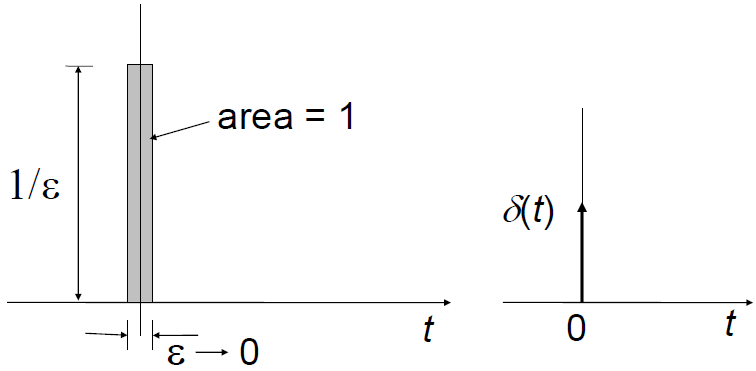
\includegraphics[width = 0.8\textwidth]{../img/diagram23.png}
\end{figure}
The Dirac delta function is a non-physical, singularity function with the follow definition:
\begin{equation}
  \delta (t) = \begin{cases}
    0 \textrm{ for } t \neq 0\\
    \textrm{undefined for } t = 0 
  \end{cases}
\end{equation}
but with the requirement that
\begin{equation}
  \int_{-\infty}^{\infty} \delta (t) \,\mathrm{d}t =1
\end{equation}
so taking the Laplace transform of this is also just 1
\begin{equation}
  \mathcal{L} (\delta (t)) = \int_{0^-}^{\infty} \delta (t) e^{-st} \,\mathrm{d}t = 1 
\end{equation}
Thus, the impulse response of the system is equal to the transfer function and from this it can be shown that \textbf{any} arbitrary signal can be described as a summation of impulse responses.
\subsection{Impulse response on a first order system}
Take a first order response for example, the transfer function and thus the impulse response looks like this:
\begin{figure}[H]
  \centering
  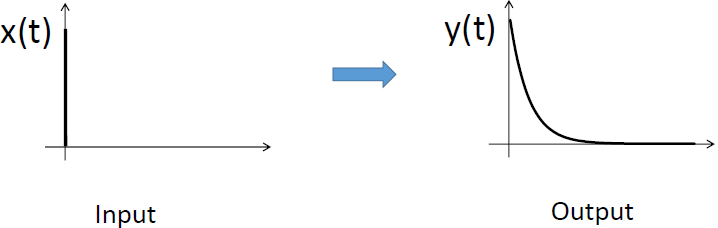
\includegraphics[width = 0.8\textwidth]{../img/diagram24.png}
\end{figure}
Due to our LTI assumptions:
\begin{itemize}
  \item Scaling the input scales the output
  \item Superposition of inputs equals superposition of outputs
  \item Time invariance
\end{itemize}
\subsection{Impulse response of a system}
\begin{figure}[H]
  \centering
  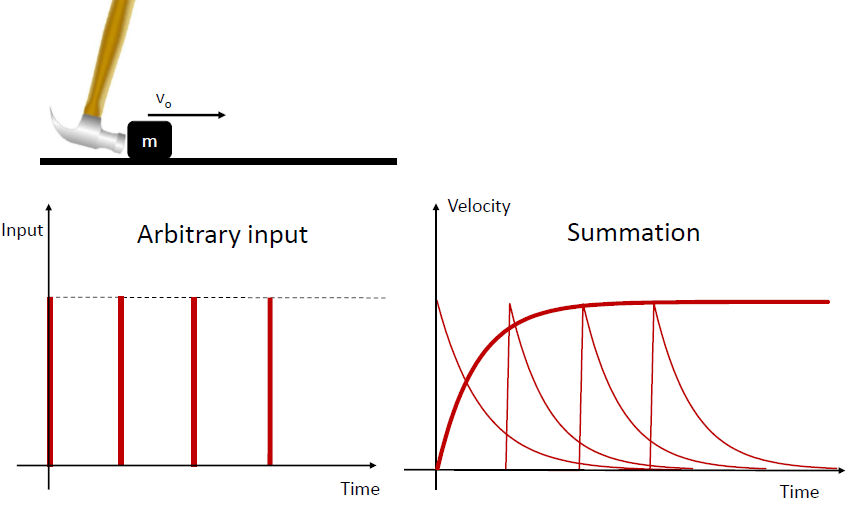
\includegraphics[width = 0.8\textwidth]{../img/diagram25.png}
\end{figure}
\subsubsection{Time vs Frequency Domain}
\begin{figure}[H]
  \centering
  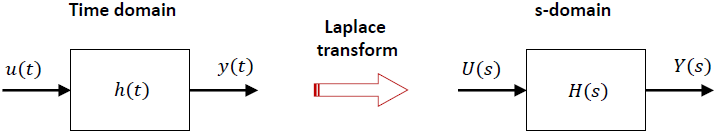
\includegraphics[width = 0.8\textwidth]{../img/diagram26.png}
\end{figure}
\begin{itemize}
  \item $u$ is the impulse function to the system
  \item $h$ is called the impulse response of the system
  \item $H$ is called the transfer function (TF) of the system
\end{itemize}
\begin{equation}
  y(t) = \int_{0}^{\infty} h(\tau) u (t-\tau) \,\mathrm{d}\tau = \int_{0}^{\infty} h(\tau - t)u(\tau) \,\mathrm{d}\tau  
\end{equation}
with $0\leq \tau \leq t$
\begin{equation}
  y(t) = h(t) \cdot u(t)
\end{equation}
This is called convolution.
\begin{equation}
  Y(s) = H(s) \cdot U(s)
\end{equation}
This is called multiplication.
\subsubsection{Convolution example}
Essentially, the steps for convolving two signals are to first reflect the signal $g$, then offset the reflected signal. Then calculate the area under the graph for every offset, by sliding $-g$. The convolution at each time point is equal to the area under the intersection of functions. For two pulses, the result is a triangle wave:
\begin{figure}[H]
  \centering
  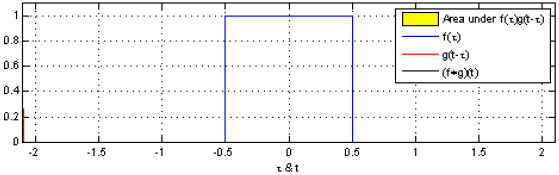
\includegraphics[width = 0.8\textwidth]{../img/diagram27.png}
\end{figure}
However, the calculations to obtain this result in the time domain are complicated, but are only multiplication in the Laplace domain.
\subsubsection{Getting the Time Response}
The procedure to describe the time response for LTI systems is thus:
\begin{itemize}
  \item Express the input, $u(t)$, in Laplace notation, $U(s)$
  \item Use this to find output $Y(s)$, usually by multiplying $U(s)$ by the transfer function $Y(s) = U(s)G(s)$
  \item Use inverse Laplace transforms (from tables) to express $Y(s)$ as a function of time, $y(t)$
\end{itemize}
\section{Input functions: Impulse - Step - Ramp}
Now we will consider some standard inputs and look at the response of first and second order systems:
\begin{itemize}
  \item Impulse
  \begin{itemize}
    \item The Laplace transform is 1, so the response to an impulse is by the definition the transfer function
  \end{itemize}
  \item Step
  \item Ramp
\end{itemize}
There are many others, particularly sinusoidal inputs or other discontinuous inputs, which are important in control loops, but we will focus on the two classic examples.
\subsection{Step input}
A step input is a discontinuous function, which is zero for all negative values of $t$ and 1 for all positive values.
\begin{figure}[H]
  \centering
  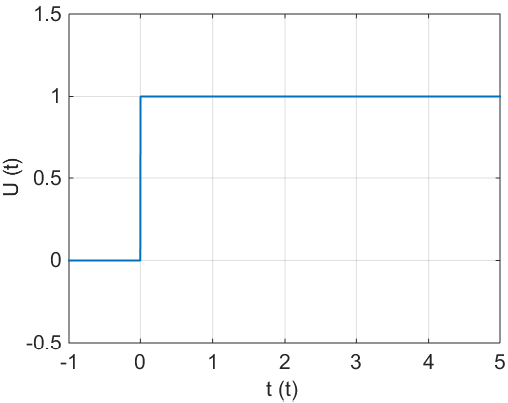
\includegraphics[width = 0.8\textwidth]{../img/diagram28.png}
\end{figure}
\subsubsection{Laplace transform}
\begin{gather}
  x(t) = U(t)\\
  \mathcal{L} \left\{ U(t) \right\} = \int_{0^-}^{\infty} e^{-st} \,\mathrm{d}t = \left[-\frac{1}{s} e^{-st}\right]_{0^-}^{\infty} \rightarrow \frac{1}{s}\\    
\end{gather}
Or for a gain of A
\begin{gather}
  x(t) = AU(t) \\
  \mathcal{L} \left\{ AU(t) \right\} = \frac{A}{s} 
\end{gather}
\subsubsection{Applications}
The step response is extremely useful in control theory for describing the behaviour of the system. In part because it incorporates the "transient" behaviour - from the sudden change from zero to one, as well as the "steady state" behaviour as the system settles down to a single value. IT also replicates many real world control applications such as:
\begin{itemize}
  \item Position control - move to a $X=10\si{\milli\meter}$ position and stay
  \item Speed control - go to 33 RPM
  \item Temperature - heat element on 3D printer to 230 \si{\celsius}
\end{itemize}
Also, unlike the Dirac impulse - it is physically realisable.
\subsection{Ramp input}
A ramp input has a value of $t$ for all $t$ values above zero and zero elsewhere, often is scaled by a gain A.
\begin{figure}[H]
  \centering
  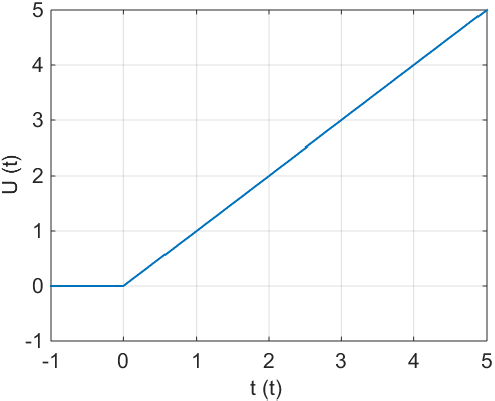
\includegraphics[width = 0.8\textwidth]{../img/diagram29.png}
\end{figure}
\subsubsection{Laplace transform}
\begin{gather}
  x(t) = at\\
  \mathcal{L} \left\{ at \right\} \int_{0^-}^{\infty} ate^{-st} \,\mathrm{d}t = -a \left[ \frac{t}{s}e^{-st} \right]_{0}^{\infty} + a\int_{0}^{\infty} \frac{1}{s} e^{-st} \,\mathrm{d}t\\
  = a \left[ -\frac{1}{s^2}e^{-st} \right] \rightarrow \frac{a}{s^2}   
\end{gather}
\subsubsection{Applications}
Ramp inputs are useful in understanding the steady state behaviour of a system i.e. when $t$ goes to infinity. Practical examples of control applications using ramp inputs are
\begin{itemize}
  \item Servo motors - shaft \textbf{position} rather than speed
  \item Ovens for PCB manufacturing etc. - strict linear \textbf{profile} of temperature required as opposed to "get to this temperature quickly"
  \item CNC milling machine, move in $X$ direction and constant rate
\end{itemize}
\end{document}